\section{Конструкторская часть}

% Кратко описать, что будет в конструкторской части

В данной части будут приведены требования к программному обеспечению, на формальном языке будут описаны алгоритмы, которые будут реализованы при разработке программного обеспечения, а также будет обоснован выбор типов и структур, которые будут использованы при разработке. %, и приведена общая архитектура разрабатываемой программы.

\subsection{Требования к программному обеспечению}

% Составить ТЗ, что должна делать программа

Разрабатываемое программное обеспечение должно предоставлять пользователю следующую функциональность:
\begin{itemize}
    \item добавление объекта на сцену (куб, сфера, чайник);
    \item выбор объекта сцены с помощью клавиатуры;
    \item изменение цвета выбранного объекта;
    \item изменение геометрических свойств выбранного объекта (положение в пространстве, поворот, увеличение);
    \item изменение физических свойств выбранного объекта (масса, скорость, ускорение, сила);
    \item изменение значения гравитации;
    \item перемещение и поворот камеры с помощью клавиатуры и мыши.
\end{itemize}

При этом разрабатываемая программа должна удовлетворять следующим требованиям:
\begin{itemize}
    \item программа должна генерировать кадр не менее, чем за $\frac{1}{30}$ секунды при сцене, состоящей не более, чем из 10 объектов и размере окна 1920x1080 пикселей;
    \item никакие действия пользователя не должны приводить к аварийному завершению программы.
\end{itemize}

\subsection{Разработка алгоритмов}

Далее на формальном языке будут описаны алгоритмы, которые будут реализованы при разработке проргаммного обеспечения.

\subsubsection{Общий алгоритм работы программы}

Далее представлен общий алгоритм работы разрабатываемого программного обеспечения.

\begin{enumerate}
    \item Инициализировать используемые объекты (окно, камера, сцена, объекты сцены, графический интерфейс, шейдерная программа).
    \item Пока приложение запущено:
        \begin{itemize}
            \item обработать события от мыши и клавиатуры;
            \item обнаружить и разрешить коллизии;
            \item обновить местоположения объектов сцены;
            \item сгенерировать и отобразить кадр.
        \end{itemize}
    \item Освободить ресурсы.
\end{enumerate}

% \subsubsection{Алгоритм, использующий z-буфер}

\subsubsection{Алгоритм AABB}

На рисунке \ref{fig:aabb} представлена схема алгоритма AABB обнаружения коллизий.

\begin{figure}[H]
	\centering
	% 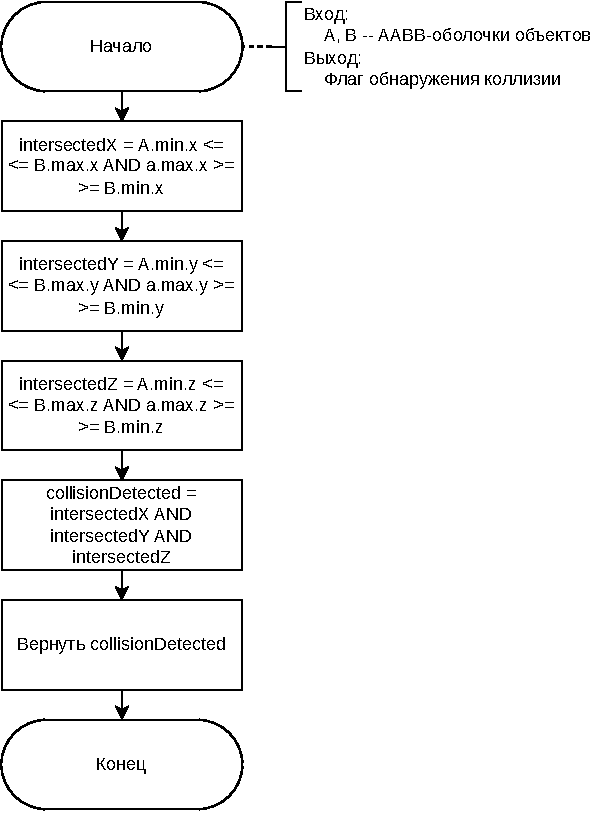
\includegraphics[scale=1]{diag/aabb.pdf}
	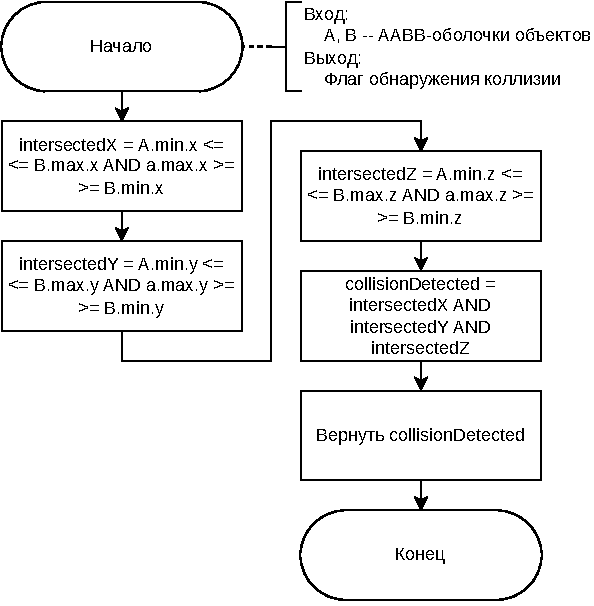
\includegraphics[scale=1]{diag/aabb_tighter.pdf}
	\caption{Алгоритм AABB обнаружения коллизий}
	\label{fig:aabb}
\end{figure}

% \subsubsection{Алгоритм GJK}

% \subsubsection{Алгоритм EPA}

\subsubsection{Модель освещения Фонга}

В модели освещения Фонга \cite{realphong, phong} учитываются три составляющих отражённого света:
\begin{enumerate}
    \item рассеянная,
    \item фоновая,
    \item зеркальная.
\end{enumerate}

\subsubsection*{Рассеянный свет}

Рассеянный свет является светом, отражаемым во всех направлениях, и его интенсивность во всех направлениях постоянна, следовательно, для его рассчёта не требуется учитывать направление взгляда камеры, но должен быть известен угол между направлением света и нормалью к поверхности объекта \cite{phong}.

\begin{figure}[H]
	\centering
	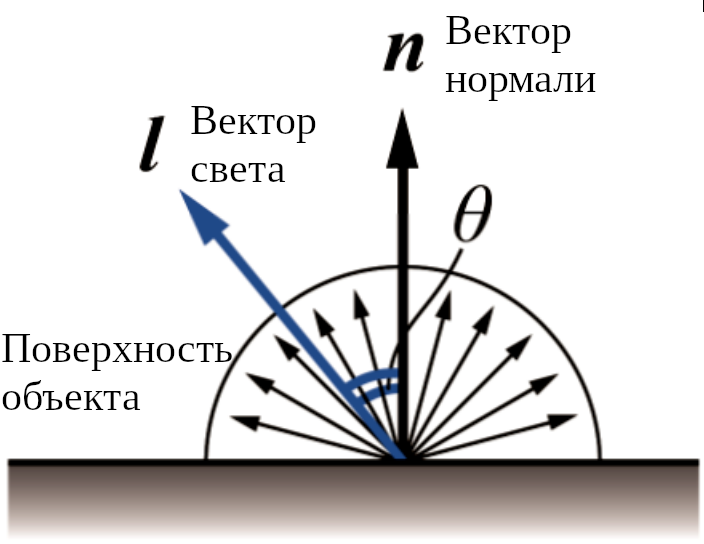
\includegraphics[width=0.56\textwidth]{img/diffuse_ru}
    \caption{Модель Фонга: Рассеянная составляющая света (Источник: \cite{phong})}
	\label{fig:diffuse}
\end{figure}

Рассеянная составляющая света, согласно \cite{phong}, рассчитывается по формуле~\ref{eq:diffuse}, приведённой ниже.

\begin{equation}
    I_d = k_d I_l \cos \theta = k_d I_l \left| \boldsymbol{n} \cdot \boldsymbol{l} \right|,
    \label{eq:diffuse}
\end{equation}
где 
\begin{itemize}
    \item $I_l$ --- интенсивность источника света,
    \item $k_d$ --- коэффициент рассеивания света,
    \item $\boldsymbol{n}$ --- вектор нормали к поверхности объекта,
    \item $\boldsymbol{l}$ --- вектор направления света,
    \item $\cos \theta$ --- угол между вектором направления света и нормалью к поверхности объекта.
\end{itemize}

\subsubsection*{Фоновое освещение}

Если учитывать только рассеяный свет при освещении объекта, будут видны абсолютно неосвещённые, чёрные грани.
В реальном мире такое встречается редко, в связи с чем, для достижения большей реалистичности, было предложено ввести минимальный уровень освещённости --- фоновое освещение, являющееся обычно результатом отражения света от других объектов сцены~\cite{phong, quakecon}.

\begin{figure}[H]
	\centering
	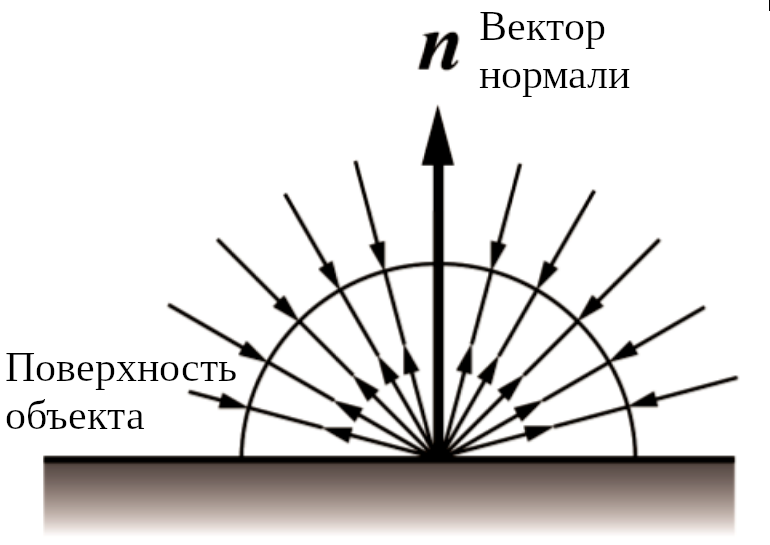
\includegraphics[width=0.6\textwidth]{img/ambient_ru}
    \caption{Модель Фонга: Фоновая составляющая света (Источник: \cite{phong})}
	\label{fig:ambient}
\end{figure}

Фоновая составляющая света, согласно \cite{phong}, рассчитывается по формуле~\ref{eq:ambient}, приведённой ниже.
\begin{equation}
    I_a = k_a I_0,
    \label{eq:ambient}
\end{equation}
где
\begin{itemize}
    \item $k_a$ --- отражательная способность объекта,
    \item $I_0$ --- интенсивность фонового освещения.
\end{itemize}

\subsubsection*{Зеркальный свет}

В реальном мире гладкие объекты отражают свет подобно зеркалу --- чем менее объект шероховатый, тем более отчётливо он отражает источник света, и виден блик.
Для достижения подобного эффекта было предложено использовать функцию косинуса и регулировать размытость границ блика с помощью возведения косинуса угла между вектором взгляда и отражённым светом в различные степени \cite{quakecon}.

\begin{figure}[H]
	\centering
	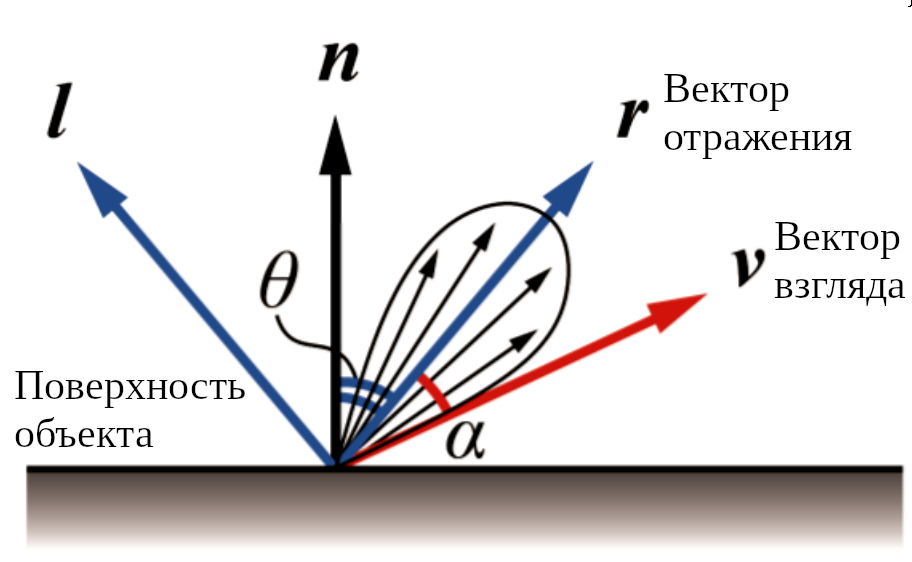
\includegraphics[width=0.66\textwidth]{img/specular_ru}
    \caption{Модель Фонга: Зеркальная составляющая света (Источник: \cite{phong})}
	\label{fig:specular}
\end{figure}

Зеркальная составляющая света, согласно \cite{phong}, рассчитывается по формуле~\ref{eq:specular}, приведённой ниже.
\begin{equation}
    I_s = k_s I_l \cos^n \alpha = k_s I_l \left| \boldsymbol{r} \cdot \boldsymbol{v} \right|^n,
    \label{eq:specular}
\end{equation}
где
\begin{itemize}
    \item $k_s$ --- коэффициент зеркального отражения,
    \item $\boldsymbol{r}$ --- вектор отражённого света,
    \item $\boldsymbol{v}$ --- вектор взгляда,
    \item $\cos \alpha$ --- угол между вектором взгляда и вектором отражённого света,
    \item $n$ --- коэффициент шероховатости поверхности.
\end{itemize}

Сумма рассеянной, фоновой и зеркальной составляющих даёт итоговый отражённый свет:
\begin{equation}
    I = k_d I_l \left| \boldsymbol{n} \cdot \boldsymbol{l} \right| + k_a I_0 + k_s I_l \left| \boldsymbol{r} \cdot \boldsymbol{v} \right|^n
    \label{eq:phong}
\end{equation}

% \subsubsection{Шаги графического конвейера}

\subsection{Выбор типов и структур данных}

% \subsection{Общая архитектура разрабатываемой программы}
% Классы

Далее будут выбраны типы и структуры данных для представления объектов в разрабатываемой программе.

\noindent
% \begin{table}[H]
    % \caption{Выбор типов и структур данных для представления объектов}
    % \label{tab:tds}
% \begin{adjustbox}{width=1\textwidth}
    % \begin{tabular}{|p{.30\textwidth}|p{.70\textwidth}|}
    \begin{longtable}{|p{.30\textwidth}|p{.65\textwidth}|}
        \caption{Выбор типов и структур данных для представления объектов \label{tab:tds}} \\
        \hline
        Объект / структура
        &
        Представление / тип данных
        \\
        \hline
        Сцена
        &
        Структура Scene с полями:
        \begin{itemize}
            \item objects типа массив структур Object (для хранения всех объектов сцены).
        \end{itemize}
        \\
        \hline
        Объект сцены
        &
        Структура Object с полями:
        \begin{itemize}
            \item mesh типа структура Mesh (для хранения информации о геометрии объекта),
            \item transform типа структура Transform (для хранения информации о положении объекта в пространстве),
            \item color типа структура Vec3 (для хранения информации о цвете объекта),
            \item collider типа структура AABB (для хранения информации о коллайдере объекта),
            \item rigidbody типа структура RigidBody (для хранения информации о физических свойствах объекта).
        \end{itemize}
        \\

        \hline
        \newpage
        \caption{Выбор типов и структур данных для представления объектов} \vspace{0.3cm} \\

        \hline
        Структура Mesh
        &
        Структура Mesh с полями:
        \begin{itemize}
            \item vertices типа массив структур Vertex (для хранения информации о вершинах объекта).
        \end{itemize}
        \\
        \hline
        Структура Vertex
        &
        Структура Vertex с полями:
        \begin{itemize}
            \item position типа структура Vec3 (для хранения информации о координатах вершины),
            \item normal типа структура Vec3 (для хранения информации о нормали к вершине).
        \end{itemize}
        \\
        \hline
        Структура Vec3
        &
        Структура Vec3 с полями:
        \begin{itemize}
            \item x типа число с плавающей точкой,
            \item y типа число с плавающей точкой,
            \item z типа число с плавающей точкой.
        \end{itemize}
        \\
        \hline
        Структура Transform
        &
        Структура Transform с полями:
        \begin{itemize}
            \item position типа структура Vec3 (для хранения информации о смещении объекта в пространстве),
            \item rotation типа структура Vec3 (для хранения информации о повороте объекта),
            \item scale типа структура Vec3 (для хранения информации о масштабировании объекта).
        \end{itemize}
        \\
        \hline

        \hline
        \newpage
        \caption{Выбор типов и структур данных для представления объектов} \vspace{0.3cm} \\

        \hline
        Структура AABB
        &
        Структура AABB с полями:
        \begin{itemize}
            \item min типа структура Vec3 (для хранения информации о вершине ограничивающего параллелепипеда с минимальными координатами по трём осям),
            \item max типа структура Vec3 (для хранения информации о вершине ограничивающего параллелепипеда с максимальными координатами по трём осям).
        \end{itemize}
        \\
        \hline
        Структура RigidBody
        &
        Структура RigidBody с полями:
        \begin{itemize}
            \item velocity типа структура Vec3 (для хранения информации о скорости объекта),
            \item acceleration типа структура Vec3 (для хранения информации об ускорении объекта),
            \item force типа структура Vec3 (для хранения информации о силе, действующей на объект),
            \item mass типа число с плавающей точкой (для хранения информации о массе объекта).
        \end{itemize}
        \\

        \hline
        \newpage
        \caption{Выбор типов и структур данных для представления объектов} \vspace{0.3cm} \\

        \hline
        Камера
        &
        Структура Camera с полями:
        \begin{itemize}
            \item position типа структура Vec3 (для хранения информации о местоположении камеры),
            \item front типа структура Vec3 (для хранения информации, нужной для рассчёта направления вектора взгляда камеры),
            \item up типа структура Vec3 (для хранения информации, нужной для рассчёта направления вектора взгляда камеры),
            \item yaw типа число с плавающей точкой (для хранения информации о повороте камеры),
            \item pitch типа число с плавающей точкой (для хранения информации о повороте камеры),
            \item fov типа число с плавающей точкой (для хранения информации о соотношении сторон камеры).
        \end{itemize}
        \\
        \hline
    % \end{tabular}
    \end{longtable}
% \end{adjustbox}
% \end{table}

\subsection{Вывод}

В данной части были приведены требования к программному обеспечению, на формальном языке были описаны алгоритмы, которые будут реализованы при разработке программного обеспечения, а также был обоснован выбор типов и структур, которые будут использованы при разработке. %, и приведена общая архитектура разрабатываемой программы.
